\title{[Lab7] Temporal Difference Learning}
\author{0616014 楊政道}
\maketitle
\thispagestyle{fancy}
\section{Report}
\subsection{A plot shows episode scores of at least 100,000 training episodes.}
\begin{figure}[!ht]
    \begin{center}
        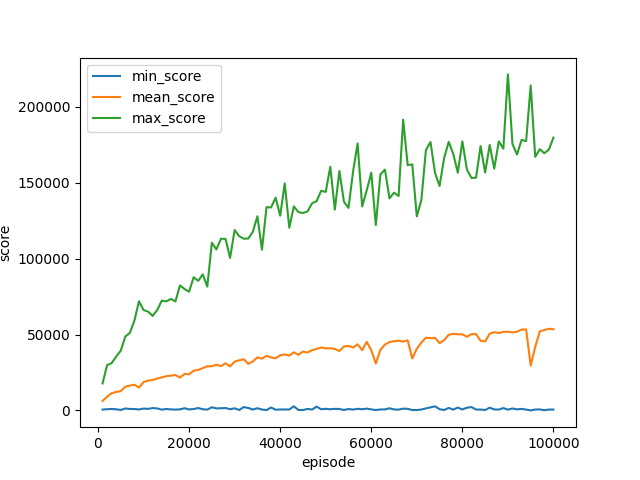
\includegraphics[width=10cm]{score_plt.png}
        \caption{Performance}
    \end{center}
\end{figure}
\subsection{Describe your implementation in detail.}
\begin{lstlisting}
\subsubsection{pattern::estimate}
virtual float estimate(const board& b) const {
    // TODO
    float ret_value = 0;
    for (int i = 0 ; i < iso_last ; i++) {
        int idx = indexof(isomorphic[i], b);
        ret_value += operator[](idx);
    }
    return ret_value;
}
\end{lstlisting}
\paragraph{}
計算一個pattern在一個board上的數值總和, 輸入會給定一個board, 要加上這個pattern所有同構方向的所有數值,並回傳回去。
\subsubsection{pattern::update}
\begin{lstlisting}
virtual float update(const board& b, float u) {
    // TODO
    float u_mean = u / iso_last, ret_value = 0;
    for (int i = 0 ; i < iso_last ; i++) {
        int idx = indexof(isomorphic[i], b);
        operator[](idx) += u_mean;
        ret_value += operator[](idx);
    }
    return ret_value;
}
\end{lstlisting}
\paragraph{}
更新一個pattern的表的數值, 要找到所有和他同構的那些格子, 並且加上要更新的數值的平均。
\subsubsection{pattern::indexOf}
\begin{lstlisting}
size_t indexof(const std::vector<int>& patt, const board& b) const {
    // TODO
    int ret = 0;
    for (int i = 0 ; i < (int)patt.size() ; i++)
        ret |= (b.at(patt[i]) << (4 * i));
    return ret;
}
\end{lstlisting}
\paragraph{}
給定某一個pattern的編號還有一個board, 要根據pattern的編號去board中撈出數值並且拼起來, 就會得到index。
\subsubsection{learning::select\_best\_move}
\begin{lstlisting}
state select_best_move(const board& b) const {
    state after[4] = { 0, 1, 2, 3 }; // up, right, down, left
    state* best = after;
    for (state* move = after; move != after + 4; move++) {
        if (move->assign(b)) {
            // TODO
            move->set_value(move->reward() + estimate(move->after_state()));
            if (move->value() > best->value())
                best = move;
        } else {
            move->set_value(-std::numeric_limits<float>::max());
        }
        debug << "test " << *move;
    }
    return *best;
}
\end{lstlisting}
\paragraph{}
根據TD learning的更新公式, 這個move的value應該要是他這步得到的reward加上下一個state(未加入新的方塊, after\_state)的估計值。
\subsubsection{learning::update\_epsisode}
\begin{lstlisting}
void update_episode(std::vector<state>& path, float alpha = 0.1) const {
    // TODO
    float sum = 0;
    path.pop_back();
    while (path.size()) {
        state& move = path.back();
        float loss = sum - (move.value() - move.reward());
        sum = move.reward() + update(move.after_state(), alpha * loss);
        path.pop_back();
    }
}
\end{lstlisting}
\paragraph{}
跑完一個episode, 要根據這個episode中的決策路徑來更新Q table, 其中alpha就是遞減的參數。
\subsection{Describe the implementation and the usage of 𝑛-tuple network.}
\paragraph{}
n-tuple存在的理由為像是2048這種所有可能的數量太龐大, 無法每個state都開一格表格來存, 因此把整個版面切成幾個群組當成一個pattern, 對於一個版面的估計值就是這些pattern所有同構的組合的累積值。實作上會將版面上每個格子都編一個16進制的數字, 而一個pattern的組成即為幾個16進制的數字所組成的集合, 並事先預處理同構。
\subsection{Explain the TD-backup diagram of V(state).}
\paragraph{}
流程為有一個state, 選擇了一個action, 他會到一個after-state, 並且env隨機放一個方塊到一個空位到達下一個state, V(state)的更新就是加上這裡的TD error。
\subsection{Explain the action selection of V(state) in a diagram.}
\paragraph{}
action的選擇為選擇他認為最好的狀態, 衡量一個狀態的好壞使用n-tuple network。
\subsection{Explain the TD-backup diagram of V(after-state).}
\paragraph{}
流程為有一個after-state, env隨機放一個方塊到一個空位到達下一個state, 接下來我選擇了一個action, 他會到另一個after-state, V(after-state)的更新就是加上這裡的TD error。
\subsection{Explain the action selection of V(after-state) in a diagram.}
\paragraph{}
action的選擇為選擇他認為最好的狀態, 衡量一個狀態的好壞使用n-tuple network。
\subsection{Explain the mechanism of temporal difference learning.}
\paragraph{}
TD learning的機制為對於每個action都會做一次Q值參數更新, 不需要搜尋一段深度才有辦法更新, 更新的依據為現在的state Q值, 下一個state的Q值已經走這步的reward。
\subsection{Explain whether the TD-update perform bootstrapping.}
\paragraph{}
Bootstrapping為邊更新邊估計, TD learning每次的更新的依據是下一個state的估計值, 因此TD learning有bootstrapping。
\subsection{Explain whether your training is on-policy or off-policy.}
\paragraph{}
這是的training方式為off-policy, 每次都會掃過所有的action, 選擇最好的那個action來執行。
\subsection{Other discussions or improvements.}
\paragraph{}
在action選擇上可以多走幾步, 雖然會讓訓練速度變慢, 但是可以讓agent考慮的更完整, 可以讓performance有機會變高。
\section{Performance}
\subsection{The 2048-tile win rate in 1000 games.}
\begin{figure}[!ht]
    \begin{center}
        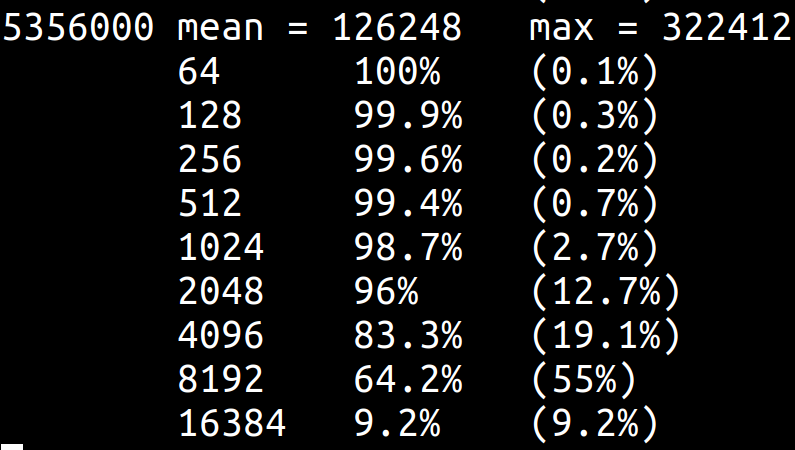
\includegraphics[width=8cm]{result.png}
        \caption{Performance}
    \end{center}
\end{figure}
